\chapter{HARDWARE CHARACTERISTICS OF A MOBILE DEVICE}\label{cha:character}\index{characteristics}
In the hardware of a device there are some features that can be used to distinguish devices from each other. In most cases it is not called features rather error sources. In the aim of this thesis it is feature characteristics that can be seen as an uniqueness of an mobile device. \textit{Device fingerprint(ing)}\index{device fingerprint} is the term used for this feature characteristics and the pyramid seen in~\figureref{fig:pyramid} from ~\cite[]{sensor:acoustic} shows the different types of sources of device fingerprint. This thesis will focus on the top of quarter of that pyramid, that is the sensors. All error sources of sensors comes in form of bias and the bias from each sensor covered by the thesis is further explained in this chapter. There is also an explanation on how the sensors is measured from Android respective JavaScript depending on the preformed tests that is described in ~\chapterref{cha:measurements}.

\begin{figure}[!h]
		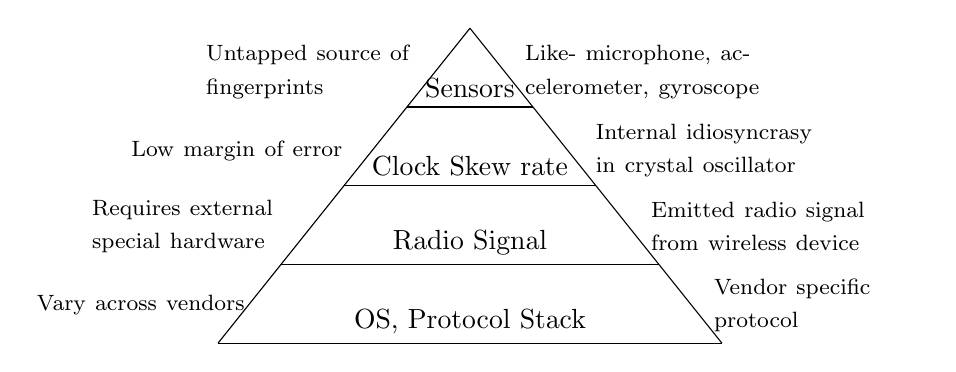
\begin{tikzpicture}[scale=1]

		\def \h {4};
		\def \f {0.8};

		\foreach \y in  {0,1,2,3} {
		    \def \w { \h*\f-\y*\f };
		    \def \v { \y*\f-\h*\f };
		    \draw (\v,\y) -- (\w,\y);
		}

		\draw (-\h*\f,0)  -- (0,\h);
		\draw (\h*\f,0)  -- (0,\h);
		\node (os) at (0,0) [above] {OS, Protocol Stack};
		\node (rf) at (0,1) [above] {Radio Signal};
		\node (cs) at (0,2) [above] {Clock Skew rate};
		\node (se) at (0,3) [above] {Sensors};


		\node [left of=os, xshift=-3cm, yshift=0.2cm, text width=3cm] {\footnotesize{Vary across vendors}};
		\node [left of=rf, xshift=-2.4cm, yshift=0.2cm, text width=2.8cm] {\footnotesize{Requires external special hardware}};
		\node [left of=cs, xshift=-1.8cm, yshift=0.2cm, text width=3cm] {\footnotesize{Low margin of error}};
		\node [left of=se, xshift=-1cm, yshift=0.2cm, text width=2.7cm] {\footnotesize{Untapped source of fingerprints}};

		\node [right of=os, xshift=3.4cm, yshift=0.2cm, text width=2.6cm] {\footnotesize{Vendor specific protocol}};
		\node [right of=rf, xshift=2.8cm, yshift=0.2cm, text width=3cm] {\footnotesize{Emitted radio signal from wireless device}};
		\node [right of=cs, xshift=2.1cm, yshift=0.2cm, text width=3cm] {\footnotesize{Internal idiosyncrasy in crystal oscillator}};
		\node [right of=se, xshift=1.3cm, yshift=0.2cm, text width=3.2cm] {\footnotesize{Like- microphone, accelerometer, gyroscope}};
	\end{tikzpicture}
	\caption{\label{fig:pyramid} The pyramid of features in a mobile device that can be used for fingerprinting.\cite[]{sensor:acoustic}}
\end{figure}

As seen above in~\figureref{fig:pyramid} are sensors an untapped source of fingerprints in mobile devices and example of sensors are microphone, accelerometer, barometer, speakers and gyroscope. The sensors investigated in this work is the accelerometer-, gyroscope-, magnetometer- and camera- sensors. All of them are common sensors in most of the mobile devices used today.


\section{Accelerometer\index{accelerometer}}\label{sec:accelerometer}
The accelerometer is the sensor that detect movement on a mobile device, like when you changing orientation on your device. Acceleration is measured by sensing how much pressure the device has in terms of force. The type of accelerometer sensor found in a mobile device is a micro-electromechanical systems known as MEMS sensor. \cite[]{sensors:fusion}
\subsection{Fingerprinting feature / Bias}
Measure the characteristics from the accelerometer is done by taking the long term average of the output when the accelerometer is in rest. That is the biggest error source in the accelerometer and it grows quadratically over time, but when the accelerometer is in rest the error $\epsilon$ can be calculated as a function of time $t$;
\begin{equation} \label{eq:AccBias}
s(t)=\epsilon * \frac{t^2}{2} 
\end{equation}
\cite[]{sensor:inertialNav}\cite[]{sensors:fusion}


\section{Gyroscope\index{gyroscope}}\label{sec:gyroscope}
The gyroscope is sensing how the device is moving in terms of angles, for maintaining or measure the orientation. This is originally  a mechanical system based on the principle of conservation of angular momentum. The most popular Gyroscope for devices today is a MEMS that is using silicon micro-mechanical techniques. Coriolis effect is measured with vibrating elements in the MEMS gyroscope. Coriolis effect is a change of moving objects direction when looking at it from a rotating reference system. The difference from the accelerometer is that the gyroscope measures relative to the device body rather than relative to earth. The equations of Coriolis force;  
$$\boldsymbol{ F}_C = -2 \, m \, (\omega *  v)$$
Where $m$ is the mass of the particle, $\omega$ the angular velocity and $v$ the velocity of the particle in the rotating system. 
\cite[]{sensor:inertialNav}
\subsection{Fingerprinting feature / Bias}
The gyroscope has some error characteristics like constant bias, white noise, bias instability, calibration error and temperature effects. One of these error characteristics that can be tested by reading the output from a gyroscope in rest is the \textit{constant bias}\index{constant bias}. That is bias of the gyroscope output when not having any rotation on it. This constant error $\epsilon$ of the bias over time $t$ leads to an angular error that grows linear; 
\begin{equation} \label{eq:gyroBias}
\theta (t)= \epsilon * t
\end{equation}
If take the long term average output from the gyro in rest, the constant error of a rate gyro can be estimated.\cite[]{sensors:fusion}


\section{Magnetometer\index{magnetometer}}
The magnetometer measures the magnetic field and was originally used for navigation and tracking. When it is used as a compass the Earth's magnetic field is measured. The type of sensor found in mobile devices is like accelerometer and gyroscope a MEMS sensor. They are known as e-compasses gaussmeters that is measuring of magnetic fields larger than 1 nT.
~\cite[]{sensor:magn}

\subsection{Fingerprinting feature / Bias}
\textit{Note that normally bias in a magnetometer is called \textbf{offset} but for uniformity reason of this report it will be referenced to \textbf{bias}.}\\
When try to measure the magnetic field of Earth with a magnetometer it also gets affected by other magnetic fields. The two main error sources from measurements of magnetometer are magnetic contamination in the sensor, called Soft and Hard-Iron distortion. \\
The hard iron distortion is caused by metals and magnets around the magnetometer. This field is constant even if the device moves, thus it is additive to the earths magnetic field. This distortion can be caused of e.g. the device speaker mounted near the magnetometer. \\
If there are magnetic fields in the surrounding environment of the device they will cause soft iron disorder. This error is smaller than the hard iron distortion. Any metal around the device can cause this error, such a car passing by.
There are also a third bias that can effect the magnetometer and is as the hard iron distortion additive. This bias is the errors in the magnetometer itself such that all hardware has. But the result of this bias is similar to the soft iron distortion.  \\
The good thing with magnetometer bias is that it is constant over time, thus once it is calculated it stays the same. \\
\\
If the device is rotated one turn (360\degree)around its own z-axes (see~\figureref{fig:device-axes}) and plot x with respect to y there will be a circle. In a world without bias this circle will look like:
\begin{figure}[H]
\begin{tabular}{p{0.23\textwidth} p{0.23\textwidth} p{0.23\textwidth} p{0.23\textwidth}}
        \vspace{0pt} \begin{tikzpicture}[line cap=round,line join=round,>=triangle 45,x=1.0cm,y=1.0cm]
\draw[->,color=black] (-1.5,0.) -- (1.5,0.);
\foreach \x in {-1.4,-1.2,-1.,-0.8,-0.6,-0.4,-0.2,0.2,0.4,0.6,0.8,1.,1.2,1.4}
\draw[shift={(\x,0)},color=black] (0pt,-2pt);
\draw[color=black] (1.3548383992423667,0.012646598999199708) node [anchor=south west] {X};
\draw[->,color=black] (0.,-1.5) -- (0.,1.5);
\foreach \y in {-1.4,-1.2,-1.,-0.8,-0.6,-0.4,-0.2,0.2,0.4,0.6,0.8,1.,1.2,1.4}
\draw[shift={(0,\y)},color=black] (-2pt,0pt);
\draw[color=black] (0.015808248748999637,1.4306334471160802) node [anchor=west] {Y};
\clip(-1.5,-1.5) rectangle (1.5,1.5);
\draw(0.,0.) circle (1.cm);
\begin{scriptsize}
\draw [color=xdxdff] (0.,0.)-- ++(-2.0pt,-2.0pt) -- ++(4.0pt,4.0pt) ++(-4.0pt,0) -- ++(4.0pt,-4.0pt);
\draw [fill=qqqqff] (0.,1.) circle (1.5pt);
\draw[color=qqqqff] (-0.15,1.1) node {0\textrm{\degre}};
\end{scriptsize}
\end{tikzpicture}
 & 
        \vspace{0pt} \begin{tikzpicture}[line cap=round,line join=round,>=triangle 45,x=1.0cm,y=1.0cm]
\draw[->,color=black] (-1.5,0.) -- (1.5,0.);
\foreach \x in {-1.4,-1.2,-1.,-0.8,-0.6,-0.4,-0.2,0.2,0.4,0.6,0.8,1.,1.2,1.4}
\draw[shift={(\x,0)},color=black] (0pt,-2pt);
\draw[color=black] (1.3548383992423672,0.012646598999199708) node [anchor=south west] {X};
\draw[->,color=black] (0.,-1.5) -- (0.,1.5);
\foreach \y in {-1.4,-1.2,-1.,-0.8,-0.6,-0.4,-0.2,0.2,0.4,0.6,0.8,1.,1.2,1.4}
\draw[shift={(0,\y)},color=black] (-2pt,0pt);
\draw[color=black] (0.015808248748999637,1.4306334471160802) node [anchor=west] {Y};
\clip(-1.5,-1.5) rectangle (1.5,1.5);
\draw(-0.2,-0.2) circle (1.003958800671448cm);
\begin{scriptsize}
\draw [fill=qqqqff] (-0.18558461983368865,0.8038553034478191) circle (1.5pt);
\draw[color=qqqqff] (-0.16,1) node {0\textrm{\degre}};
\draw [color=xdxdff] (-0.2,-0.2)-- ++(-2.0pt,-2.0pt) -- ++(4.0pt,4.0pt) ++(-4.0pt,0) -- ++(4.0pt,-4.0pt);
\end{scriptsize}
\end{tikzpicture} & 
        \vspace{0pt} \begin{tikzpicture}[line cap=round,line join=round,>=triangle 45,x=1.0cm,y=1.0cm]
\draw[->,color=black] (-1.5002742877331638,0.) -- (1.5002742877331638,0.);
\foreach \x in {-1.4,-1.2,-1.,-0.8,-0.6,-0.4,-0.2,0.2,0.4,0.6,0.8,1.,1.2,1.4}
\draw[shift={(\x,0)},color=black] (0pt,-2pt);
\draw[color=black] (1.3548383992423672,0.012646598999199708) node [anchor=south west] {X};
\draw[->,color=black] (0.,-1.500215870948452) -- (0.,1.5001897416116785);
\foreach \y in {-1.4,-1.2,-1.,-0.8,-0.6,-0.4,-0.2,0.2,0.4,0.6,0.8,1.,1.2,1.4}
\draw[shift={(0,\y)},color=black] (-2pt,0pt);
\draw[color=black] (0.015808248748999637,1.4306334471160802) node [anchor=west] {Y};
\clip(-1.5002742877331638,-1.500215870948452) rectangle (1.5002742877331638,1.5001897416116785);
\draw [rotate around={-36.86989764584405:(0.,-0.15)}] (0.,-0.15) ellipse (1.1608455676650522cm and 0.8860374890305703cm);
\begin{scriptsize}
\draw [color=xdxdff] (0.04907705257499707,-0.12173658003568395)-- ++(-2.0pt,-2.0pt) -- ++(4.0pt,4.0pt) ++(-4.0pt,0) -- ++(4.0pt,-4.0pt);
\draw [fill=qqqqff] (-0.8962562226151813,0.5864729639194997) circle (1.5pt);
\draw[color=qqqqff] (-1.1,0.75) node {0\textrm{\degre}};
\end{scriptsize}
\end{tikzpicture} & 
        \vspace{0pt} \begin{tikzpicture}[line cap=round,line join=round,>=triangle 45,x=1.0cm,y=1.0cm]
\draw[->,color=black] (-1.500130470417328,0.) -- (1.5002743955178048,0.);
\foreach \x in {-1.4,-1.2,-1.,-0.8,-0.6,-0.4,-0.2,0.2,0.4,0.6,0.8,1.,1.2,1.4}
\draw[shift={(\x,0)},color=black] (0pt,-2pt);
\draw[color=black] (1.3548385432174719,0.012646598999199708) node [anchor=south west] {X};
\draw[->,color=black] (0.,-1.500215870948452) -- (0.,1.5001897416116785);
\foreach \y in {-1.4,-1.2,-1.,-0.8,-0.6,-0.4,-0.2,0.2,0.4,0.6,0.8,1.,1.2,1.4}
\draw[shift={(0,\y)},color=black]  (-2pt,0pt);
\draw[color=black] (0.015808244815253596,1.4306334471160802) node [anchor=west] {Y};
\clip(-1.500130470417328,-1.500215870948452) rectangle (1.5002743955178048,1.5001897416116785);
\draw [rotate around={0.059845574260994405:(4.8164851529053886E-4,7.838801032565946E-4)}] (4.8164851529053886E-4,7.838801032565946E-4) ellipse (1.2496624710485813cm and 0.9992161789727994cm);
\begin{scriptsize}
\draw [color=xdxdff] (0.,0.)-- ++(-2.0pt,-2.0pt) -- ++(4.0pt,4.0pt) ++(-4.0pt,0) -- ++(4.0pt,-4.0pt);
\draw [fill=qqqqff] (0.,1.) circle (1.5pt);
\draw[color=qqqqff] (-0.15,1.1) node {0\textrm{\degre}};
\end{scriptsize}
\end{tikzpicture} \\
        \vspace{0pt} Ideal & Hard Iron distortion & Soft Iron distortion & Gain mismatch \\
\end{tabular}
\caption{Example of different magnetometer readings when affected by bias.}\label{fig:magnCircle}
\end{figure}
\cite[]{liu:magnAcc}

\subsection{Magnetometer calibration}
To do a magnetometer calibration the device is turned 360\degree around the z-axis (~\figureref{fig:device-axes}), with the device on a flat surface. This makes x and y-axis the surface and z-axis pointing (UP/DOWN?). To calculate the offset $O_{x,y,z}$ the average of min and max-value from each axis is calculated (the center of the circle) from the magnetic field $B_{x,y,z}$, like:
\begin{subequations}
\begin{align}
  O_x = \frac{max(B_x) + min(B_x)}{2} \\
  O_y = \frac{max(B_y) + min(B_y)}{2} \\
  O_z = \frac{max(B_z) + min(B_z)}{2}
\end{align} 
And the hard iron compensated result $m_{x,y,z}^h$:
\begin{align}
  m_x^h = B_x - O_x \\
  m_y^h = B_y - O_y \\
  m_z^h = B_z - O_z
\end{align}
\end{subequations}
The soft iron is sometimes compensated for in the equations above and sometimes additional compensation has to be done. Since soft iron offset is place specific it will not be considered in the thesis since a fingerprint of a device is not convenient if you have to be at the exact same spot every time the device tries to authenticate.
\cite[]{liu:magnAcc}


\section{Camera}\label{sec:char:camera}\index{camera fingerprinting}\index{camera}
\textit{Note that normally bias in a camera sensor is called \textbf{noise} but for uniformity reason of this report it will be referenced to \textbf{bias}.}\\
\\
The digital camera of a mobile device also includes sensors and other hardware that can be used as fingerprinting characteristics. The basic is that light travels trough a lens and hits a imaging sensor which contains pixels that has a filter array in front. The filter is for gives each pixel a detected color. The pixels is then put together again to a resulting signal which is send to some final post processing (color correction, white balance, etc.) steps before the image is written to the memory card. In this process there are different kind of bias that effects the image;
\begin{itemize}
	\item[] \textit{\index{shot noise}Shot noise -} the amount of photons hitting the sensor and each pixel varies a random amount
	\item[] \textit{\index{fixed pattern noise}Fixed pattern noise - }there is a small electric current that leaks from photo-diodes in each pixel, caused by dark current
	\item[] \textit{\index{photo-response non-uniformity noise}\index{PRNU}Photo-response non-uniformity noise (PRNU) -} is a bias that is not affected by temperature or humidity. When manufacturing sensors the silicon gets imperfection which causes that pixels aren't equally sensitive to light. This is the main source of pattern bias and makes it really unlikely for two cameras to have the same pattern.
\end{itemize}
The three types of bias can be described as a mathematical model for getting the output of the sensor $y_{ij}$:
$$y_{ij}=f_{ij}(x_{ij}+\eta_{ij})+c_{ij}+\epsilon_{ij}$$
where $f_{ij}$ is a multiple factor close to one that captures PRNU, $x_{ij}$ is the number of photons hitting the sensor, $\eta_{ij}$ the shot noise, $c_{ij}$ the dark current and $\epsilon_{ij}$ the additive random bias. The key for a unique fingerprint of the camera (in the mobile device) is to finding $f$.
\cite[]{sensor:camera:DCIdent}


\section{Measurements of sensors on mobile devices}\label{sec:charMeasureSensor}
Measurements of sensors from mobile devices can be gather in different ways. In the work of this thesis two approaches is used, a browser application and an Android application. The camera is an exception where pictures provides the sensor characteristics.
\begin{figure}[H]
	\centering
    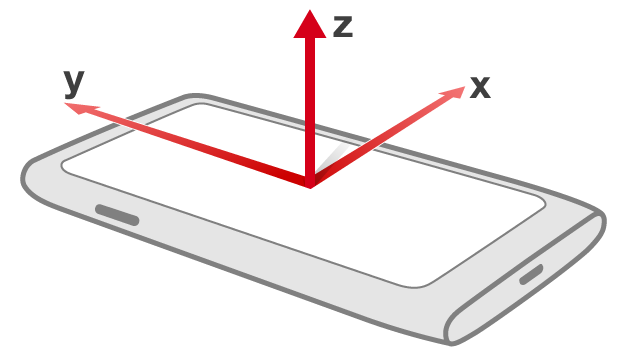
\includegraphics[scale=0.2]{img/device-axes}
    \caption{The coordinate system used for both Android and JavaScript\cite[]{sensor:W3C}}
  \label{fig:device-axes}
\end{figure}

\subsection{Android}\label{subsec:Android}\index{Android}
Android sensor framework provides raw data with high precision from sensor that are built in the device such as different motions sensors (including accelerometer and gyroscope), environmental sensors and position sensors (e.g. magnetometer). \cite[]{android:sensor}
Android sensor framework classes that is used for gather sensor data is; 
\begin{itemize}
	\item[] \texttt{SensorManager}, a manager used to access the sensor of the device. 
	\item[] \texttt{Sensor}, representing a sensor
	\item[] \texttt{SensorEvent}, an event from a Sensor such data from the sensor, time-stamp or accuracy
	\item[] \texttt{SensorEventListener}, gets a SensorEvent when a sensor or accuracy has changed 
\end{itemize}
In Android you can't just read from the sensor whenever you need, instead the SensorEventListener has a function that is triggered every time the sensor is changed. You can however set how fast the delay from the sensor should be. The function provides the output of the sensor with a time-stamp of when (in nanoseconds) the change occured. The template code for this function:
\lstinputlisting{code/android-sensor.java}\label{code:androidSensor}
\cite[]{android:sensorEvent} 




\subsubsection{Accelerometer in Android}\label{subsec:accAndroid}
\texttt{TYPE\_ACCELEROMETER} is the hardware measurements that measures the force of acceleration including the force of gravity with the SI unit $m/s^2$. Android also provide \texttt{TYPE\_LINEAR\_ACCELERATION} that is without gravity but that is a combined hardware and software sensor, thus this tests uses  \texttt{TYPE\_ACCELEROMETER} that provides almost raw data. There have been some bias removal from the sensor such bias from different temperature. \\
To get the acceleration applied to the device ($a_d$) the measurements of the force ($F_s$) applied the sensor is calculated from Newtons second law using the mass ($m$) of the device :
$$a_d=-\sum F_s / m $$ 
These measurements from the \texttt{SensorEvent} is in the x-,y- and z-axes like in~\figureref{fig:device-axes} and collected from event like x=a, y=b and z=c in~\ref{code:androidSensor}. \cite[]{android:sensorEvent}


\subsubsection{Gyroscope in Android}\label{subsec:gyroAndroid}
The data from the gyroscope sensor is collected from the \texttt{TYPE\_GYROSCOPE} that measures the rotation in rad/s around the x-, y- and z-axis of~\figureref{fig:device-axes}. The direction of the rotation is positive counter-clockwise if looking from a positive location of the axes. The values from the measurements when the gyroscope is changed is given like rotation in x=a, y=b and z=c in~\ref{code:androidSensor}. Additional output is \texttt{values[3], values[4]} and \texttt{values[5]} that is the estimated drift arounf the axis in also in rad/s.\\
Android also provide a \texttt{TYPE\_GYROSCOPE\_UNCALIBRATED} that is the same as \texttt{TYPE\_GYROSCOPE} except that no drift has been compensated for. There is still factory calibration and temperature compensation applied. \cite[]{android:sensorEvent} This makes it possible to calculate the linear sensor bias (equation~\ref{eq:gyroBias}] without Androids own bias compensation that is not known what it is.



\subsubsection{Magnetometer in Android}\label{subsec:magnAndroid}
Measures the magnetic field in x-, y- and z-axis in micro-Tesla ($\mu T$), as for the other sensors is that output for \texttt{values[0], values[1]} and \texttt{values[2]} (see code~\ref{code:androidSensor}). Android also provides a uncalibrated version that not has any calibration for the hard iron calibration. The uncalibrated type in Android is \texttt{TYPE\_MAGNETIC\_FIELD\_UNCALIBRATED} and as for the gyrocope it also comes with an bias estimation in x, y and z-axis for event-values \texttt{values[3], values[4]} and \texttt{values[5]}. 

\subsubsection{Fingerprinting: Sensor fusion in Android}
\url{http://www.codeproject.com/Articles/729759/Android-Sensor-Fusion-Tutorial}

\subsection{JavaScript}\label{subsec:js}\index{JavaScript}
JavaScript has since the use of smart-phones adapted a lot of new features, which makes it possible to access a lot of features in the devices. To access the gyroscope and accelerometer-data no permission from the user is needed, thus the user do not have to know that the sensors are measured.


\subsubsection{Accelerometer in JavaScript}\label{subsec:accJS}
To get measurements from the accelerometer an event listener called \texttt{devicemotion} is added. The output from measurements is the acceleration force in $m/s^2$ according to x-, y- and z-axes as in~\figureref{fig:device-axes}. \\
\\
In JavaScript there are two types of acceleration, \texttt{accelerationIncludingGravity} and \texttt{acceleration}.\texttt{accelerationIncludingGravity} is acceleration made by the device. In context to \texttt{acceleration} not depending on influence of gravity only by the acceleration made on the device. Since the accelerometer in the device measures with gravity I assume that that is the most raw data you can get of the two. There is no documentation on this made, thus that makes this some kind of a guess.\\
\\
The JavaScript for measurements of the accelerometer:
\lstinputlisting{code/acc-listener.js}
\cite[]{sensor:W3C}


\subsubsection{Gyroscope in JavaScript}\label{subsec:gyroJS}
A listener is implemented in the same way as for the accelerometer, this listener is called  \texttt{deviceorientation}. The output from this listener is made in degrees of rotation angle. JavaScript has named this rotations as the~\figureref{fig:device-rot} below.
\begin{figure}[H]
  \hspace{-1cm}
  \centering
  \begin{minipage}[c]{.23\textwidth}
    \centering
    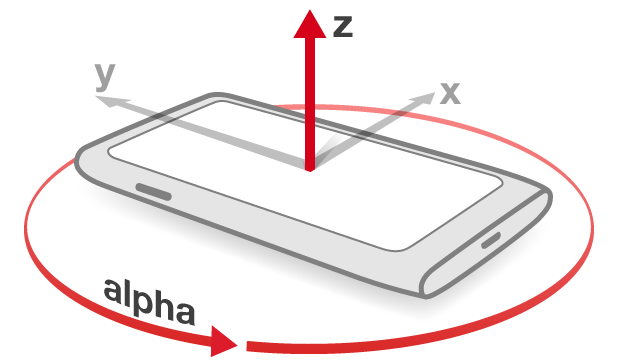
\includegraphics[scale=0.2]{img/device-alpha}
  \end{minipage}
  \hspace{1cm}
  \begin{minipage}[c]{.23\textwidth}
    \centering
    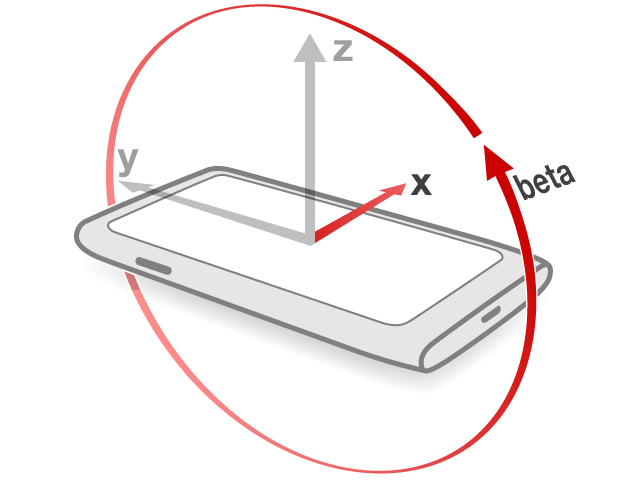
\includegraphics[scale=0.2]{img/device-beta}
  \end{minipage}
  \hspace{1cm}
  \begin{minipage}[c]{.23\textwidth}
    \centering
    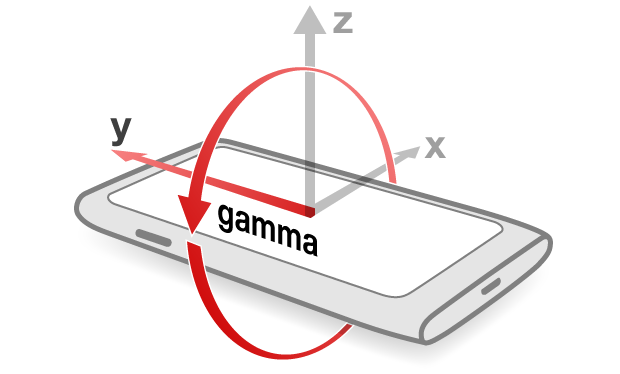
\includegraphics[scale=0.2]{img/device-gamma}
    \hspace{1cm}
  \end{minipage}
  \caption{The device rotation axes for the JavaScript \texttt{DeviceOrientation}}
  \label{fig:device-rot}
\end{figure}
Alpha is measured in the range of 0\degree to 360\degree around the z-axis, beta in in the range of -180\degree to 180\degree around x-axis and gamma in the range of -90\degree to 90\degree around y-axis.\\
\\
The JavaScript for measurements of the gyroscope:
\lstinputlisting{code/gyro-listener.js}
\cite[]{sensor:W3C}
